\chapter{Morse-Funktionen und Pseudo-Gradienten}

Das Ziel dieses Kapitels ist es, Morse-Funktionen und Pseudo-Gradienten zu
definieren und ihre \todo{allgegen- wertigkeit ist nicht so ein schönes Wort}
\textit{allgegenwertigkeit} zu zeigen. Ein weiteres wichtiges Ergebnis ist
das \textit{Morse-Lemma}.

\section{Morse-Funktionen}

In diesem Abschnitt untersuchen wir \textit{Morse-Funktionen}:

\begin{definition}[Morse-Funktion]
    \label{def: morse-funktion}
    Eine \textit{Morse-Funktion} auf einer glatten Mannigfaltigkeit $M$ ist eine glatte Funktion
    $f \colon M \to \R$, deren kritische Punkte alle nicht degeneriert sind.
\end{definition}

Insbesondere zeigen wir, dass Morse Funktionen nichts besonderes sind. Dafür zeigen wir, dass für 
eine Untermannigfaltigkeit $M \subseteq \R^n$ und einen Punkt $p \in \R^n$ die Abbildung
$x \mapsto \| x - p \|^2$ nur für $p$, die so gennanten \textit{Brennpunkte}
sind, keine Morse Funktion ist.

\begin{definition}[Normalenbündel]
    \label{def: normalenbuendel}
    Es sei $M \subseteq \R^n$ eine Untermannigfaltigkeit von $\R^n$. Das Normalenbündel ist die 
    Menge
    \[ NM = \{ (x, v) \in M \times \R^n : v \perp T_xM \} . \]
    Wir betrachten hier $T_xM \subseteq T_x\R^n \isom \R^n$ via der Basis 
    $\left( \del / \del x_i \right)$, wobei $x_i$ die Achsen des $\R^n$ sind.
\end{definition}

\begin{prop}
    \label{prop: NM ist untermannigfaltigkeit}
    Das Normalenbündel $NM$ ist eine $n$-dimensionale Untermannigfaltigkeit von $M \times \R^n$.
\end{prop}

\begin{proof}
    Es sei $x \in M$. Dann existiert eine Umgebung $U \subseteq \R^n$ von $x$, eine Umgebung 
    $\Omega \subseteq \R^d$ von $0$ und eine Immersion 
    \begin{align*}
        h \colon \Omega \longto & \R^n \\
        (u_1, \dots, u_d) \; \longmapsto & \; x(u_1, \dots, u_d)
    \end{align*}
    die ein Diffeomorphismus $h \colon \Omega \to U \cap M$ ist. Das orthogonale Komplement 
    von $T_xM$ in $\R^n$ hat Dimension $n - d$. Es sei also 
    $(v_1(x), ..., v_{n-d}(x))$ eine Basis von $(T_xM)^{\perp}$. Dann ist 
    \[ (u_1, ..., u_d, t_1, ..., t_{n - d}) \longmapsto 
        \left(x(u_1, ..., u_n), \sum_{k = 1}^{n - d} t_k \cdot v_k(u_1, ..., u_d)\right) \]
    eine lokale Parametrisierung von $NM$ als Untermannigfaltigkeit von $M \times \R^n$.
\end{proof}

\begin{definition}[Brennpunkt]
    \label{def: brennpunkt}
    Es sei $M \subseteq \R^n$ eine Untermannigfaltigkeit von $\R^n$. Es sei $E \colon NM \to R^n$ 
    mit $E (x, v) = x + v$. Ein \textit{Brennpunkt} von $M$ ist ein kriticher Wert von $E$.
\end{definition}

\begin{remark}
    Aus dem Satz von Sard folgt, dass die Menge der Brennpunkte eine Nullmenge ist.
    Intuitiv sind die Brennpunkte einer Untermannigfaltigkeit die Punkte im $\R^n$, an denen sich
    die Normalen von nahe aneinanderliegenden Punkten schneiden.
\end{remark}

\begin{lemma}
    \label{lemma: char. von Brennpunkten}
    Es sei $M \subseteq \R^n$ eine Untermannigfaltigkeit von $\R^n$ $x \in M$ und $M$ in einer 
    Umgebung von $x$ und $NM$ parametriesiert wie im Beweis von 
    Proposition~\ref{prop: NM ist untermannigfaltigkeit}. Dann ist $p = x + v$ genau dann ein
    Brennpunkt von $M$, wenn die Matrix 
    \[
        \left( \left\langle \pderive[x]{u_j}, \pderive[x]{u_i} \right\rangle - 
        \left\langle v , \pdderive[x]{u_i}{u_j} \right\rangle \right)_{ij}
    \]
    nicht invertierbar ist.
\end{lemma}

\begin{proof}
    Wir haben partielle Ableitungen
    \[ \pderive[e]{u_i} = \pderive[x]{u_i} + \sum_{k = 1}^{n - d} t_k \pderive[v_k]{u_i} \]
    und 
    \[ \pderive[E]{t_j} = v_j \]
    Nun ein kleines Ergebnis aus der Linearen Algebra:

    sind $v_1, ..., v_n, u_1, ..., u_n \in \R^n$ und $u_1, ..., u_n$ linear unabhängig, 
    dann ist
    \[ (v_1 \; ... \; v_n)^T \cdot (u_1 \; ... \; u_n) = (\langle v_i, u_j \rangle)_{ij} , \]
    Also 
    \[ \rank (v_1 ... v_n) = \rank (\langle v_i, u_j \rangle)_{ij} . \]

    Die Vektoren $ \pderive[x]{u_1}, ..., \pderive[x]{u_d}, v_1, ..., v_{n - d}$ sind linear
    unabhängig. Außerdem ist $\pderive[x]{u_l}$ orthogonal zu $v_k$, also hat die Matrix mit 
    Einträgen die Skalarprodukte dieser linear unabhängigen Vektoren mit den obigen partiellen
    Ableitungen von $E$ die Form 
    \[
        \begin{pmatrix}
            \left( \left\langle \pderive[x]{u_i}, \pderive[x]{u_j} \right\rangle + 
                \sum_{k = 1}^{n - d} t_k 
                \left\langle \pderive[v_k]{u_i} , \pderive[x]{u_j} \right\rangle \right)_{ij} &
            \left( \sum_{k = 1}^{n - d} 
                \left\langle \pderive[v_k]{u_i}, v_j \right\rangle \right)_{ij} \\
            0 & E_{n - d}
        \end{pmatrix}
    \]
    Diese Matrix hat Rang $< n$ genau dann, wenn 
    \[ \rank \left( \left\langle \pderive[x]{u_i}, \pderive[x]{u_j} \right\rangle + 
        \sum_{k = 1}^{n - d} t_k 
        \left\langle \pderive[v_k]{u_i} , \pderive[x]{u_j} \right\rangle \right)_{ij} < d 
    , \]
    Aber da $v_k$ und $\pderive[x]{u_j}$ orthogonal aufeinander stehen gilt 
    \[ 
        0 = \pderive{u_i} \left\langle v_k, \pderive[x]{u_j} \right\rangle
        = \left\langle \pderive[v_k]{u_j}, \pderive[x]{u_i} \right\rangle 
        + \left\langle v_k, \pdderive[x]{u_i}{u_j} \right\rangle
    \]
    Also 
    \begin{align*}
        \left\langle \pderive[x]{u_i}, \pderive[x]{u_j} \right\rangle + 
                \sum_{k = 1}^{n - d} t_k 
                \left\langle \pderive[v_k]{u_i} , \pderive[x]{u_j} \right\rangle
        = & \left\langle \pderive[x]{u_i}, \pderive[x]{u_j} \right\rangle - 
        \sum_{k = 1}^{n - d} t_k 
        \left\langle v_k , \pdderive[x]{u_i}{u_j} \right\rangle \\
        = & \left\langle \pderive[x]{u_i}, \pderive[x]{u_j} \right\rangle - 
        \left\langle v , \pdderive[x]{u_i}{u_j} \right\rangle
    \end{align*}
    Es folgt die Behauptung.
\end{proof}

\begin{prop}
    \label{prop: existenz morse-funktionen}
    Es sei $M \subseteq \R^n$ eine Untermannigfaltikgeit. Für fast jeden Punkt in $\R^n$ ist
    die Funktion
    \begin{align*}
        f_p \colon M & \longrightarrow \R \\
        x & \longmapsto \| x - p \|^2
    \end{align*}
    eine Morse-Funktion.
\end{prop}

\begin{proof}
    Offensichtlich ist $f_p$ glatt. $x \in M$ ist genau dann ein kritischer Punkt von $f_p$, wenn
    $T_xM \perp (x - p)$, denn das differential von $f_p$ erweitert auf $\R^n$ ist
    \[ \opd f_p (x) = 2 (x - p). \]
    Also gilt
    \[ \opd f_p (x) (v) = \langle 2 (x - p), v \rangle . \]
    $x \in M$ ist folglich genau dann ein kritischer Punkt von $f_p$, wenn $T_xM$ orthogonal 
    zu $(x - p)$ ist.

    Bemerke, dass für eine Abbildung $f \colon \R^n \to \R$ mit $f = \langle \phi_1, \phi_2 \rangle$,
    $\phi_1, \phi_2 \colon \R^n \to \R^n$ und eine Derivation $X_p$ gilt 
    \[ X_p (f) = \langle X_p(\phi_1), \phi_2 \rangle + \langle \phi_1, X_p(\phi_2) \rangle.  \]
    Sei nun $x \in M$. Dann existiert eine Umgebung $U \subseteq \R^n$ von $x$, eine Umgebung 
    $\Omega \subseteq \R^d$ von $0$ und eine Immersion 
    \[ h \colon \Omega \longto \R^n , \]
    die ein Diffeomorphismus $h \colon \Omega \to U \cap M$ ist.
    Schreibe
    \[ h(u_1, ..., u_n) = x(u_1, ..., u_n). \]
    Dann bekommen wir die partiellen Ableitungen
    \[ 
        \pderive[f_p]{u_i} = \sum_{k = 1}^n \pderive[f_p]{x_k} \cdot \pderive[x_k]{u_i} 
        = \langle 2(x - p), \pderive[x]{u_i} \rangle 
    \]
    und 
    \[ 
        \pdderive[f_p]{u_i}{u_j} = 
            2 \left( \left\langle \pderive[x]{u_j}, \pderive[x]{u_i} \right\rangle + 
            \left\langle x - p , \pdderive[x]{u_i}{u_j} \right\rangle \right) 
    . \]
    
    Also hat nach Lemma~\ref{lemma: char. von Brennpunkten} $f_p$ in einer Umgebung von $x$ genau 
    dann nicht-degenerierte kritische Punkte, wenn $f_p$ ein Brennpunkt von $M$ ist. Mit der 
    Bemerkung nach der Definition von Brennpunkten~\ref{def: brennpunkt} folgt dann direkt die 
    Behauptung.
\end{proof}

\begin{remark}
    Mit dem Einbettungssatz von Whitney folgt dann direkt, dass es auf jeder Mannigfaltigkeit 
    $M$ viele Morse-Funktionen gibt. Wir können sogar noch eine stärkere Aussage beweisen:
\end{remark}

\begin{theorem}
    \label{satz: morse-approximation}
    Es sei $M$ eine Mannigfaltigkeit, $f \colon M \to \R$ glatt. Dann kann $f$ in jeder kompakten
    Teilmenge $K$ beliebig gut von einer Morse Funktion approximirt werden, also für jedes 
    $\eps > 0$ existiert eine Morse Funktion $g \colon K \to \R$, sodass 
    \[ \| \, f - g \, \|_{\infty} < \eps . \]
\end{theorem}

\begin{proof}
    Wir wählen eine Einbettung $h' \colon M \to \R^{n - 1}$. Dann ist 
    \[ h \colon M \longto \R^n \; ; \; h(x) = (f(x), h'(x)) \]
    eine Einbettung von $M$ in $\R^n$. Seien $c, \eps_1, \dots, \eps_n > 0$, sodass für \\
    $p = (c - \eps_1, \eps_2, \dots, \eps_n)$ die Funktion $f_p$ eine Morse Funktion ist.
    Setze nun 
    \[ g(x) = \frac{f_p(x) - c^2}{2c} . \]
    $g$ ist offensichtlich eine Morse-Funktion. Wir rechnen:
    \begin{align*}
        g(x) = & \frac{1}{2c} \left( (f(x) + c - \eps_1)^2 + (h_1(x) - \eps_2)^2 
            + \dots + (h_{n-1}(x) - \eps_n)^2 - c^2 \right) \\
        = & f(x) + \frac{f(x)^2 + \sum h_i(x)^2}{2c} - \frac{\eps_1 f(x) 
            + \sum \eps_i h_{i - 1}(x)}{c} + \sum \eps_i^2 - \eps_1
    \end{align*}
    Man kann nun $c$ beliebig groß und $\eps_1, \dots, \eps_n$ beliebig klein wählen,
    sodass $g$ beliebig nah an $f$ ist.
\end{proof}

\begin{remark}
    Die meiste Zeit werden wir uns in dieser Arbeit kompakte Mannigfaltigkeiten untersuchen,
    auf solchen kann jede glatte Funktion sogar global mit einer Morse Funktion approximieren.
\end{remark}

\section{Vektorfelder und Pseudo-Gradienten}

Wir untersuchen erst ein Paar Eigenschaften von Vektorfeldern.

\begin{definition}[Flusslinie]
    \label{def: flussliene}
    Es sei $I \subseteq \R$ ein Intervall, $M$ eine glatte Mannigfaltigkeit und  
    $\gamma \colon I  \to M$ ein glatter Weg. Dann definiere für $t_0 \in \R$
    \[ \derive[\gamma]{t} (t_0) := 
        \opd \gamma (t_0) \left( \pderive{t} \right) \in T_{\gamma(t_0)}M \]
    wobei $\pderive{t}$ das von der Indentität auf $\R$ induziertze Element in $T_t\R$ ist.

    Es sei $X \in \VFs (M)$ ein Vektorfeld auf $M$. $\gamma$ heißt Flusslinie von $X$
    falls für alle $t_0 \in \R$ gilt: 
    \[ \derive[\gamma]{t}(t_0) = X(\gamma(t_0)) . \]
\end{definition}

\begin{definition}[1-Parameter Gruppe aus Diffeomorphismen]
    \label{def: 1-parameter gruppe aus diffeos}
    Es sei $M$ eine glatte Mannigfaltigkeit. Eine 
    \textit{1-Parameter Gruppe aus Diffeomorphismen} ist eine glatte Abbildung
    \begin{align*}
        \phi \colon \R \times M \longto & \; M \\
        (t, p) \longmapsto & \; \phi_t(p)
    \end{align*}
    sodass gelten: 
    \begin{itemize}
        \item Für alle $s, t \in \R$ gilt $\phi_{s + t} = \phi_s \circ \phi_t$ und
        \item $\phi_0 = \id_{M}$.
    \end{itemize}

    Für eine 1-Parameter Gruppe aus Diffeomorphismen $\phi$ schreiben wir 
    \[ \varphi_{\bullet}(p): \R \to M ; t \mapsto \varphi_t(p) . \]

    Es sei $X \in \VFs (M)$. Eine 1-Parameter Gruppe aus Diffeomorphismen $\phi$ heißt 
    \textit{von $X$ erzeugt}, falls für alle $p \in M$ gilt:
    \[ X(p) = \derive[\phi_{\bullet}(p)]{t}(0) \]
\end{definition}

\begin{remark}
    Wie der Name suggestiert, ist für jedes $t \in \R$ $\phi_t$ ein 
    Diffeomorphismus: Das Inverse von $\phi_t$ ist $\phi_{-t}$.

    Ist außerdem $\phi$ eine von einem Vektorfeld $X$ erzeugte 1-Parameter Gruppe aus 
    Diffeomorphismen, dann sind $\phi_{\bullet}(p)$ Flusslinien von $X$:
    \begin{align*}
        X(\varphi_{t_0}(p)) 
        & = \derive[\varphi_{\bullet}(\varphi_{t_0}(p))]{t}(0)
        = \opd \varphi_{\bullet} (0) (\varphi_{t_0}(p)) \left(\derive{t}\right) \\
        & = \opd (\varphi_{t_0 + \bullet}(p)) (0) \left(\derive{t}\right)
        = \opd (\varphi_{\bullet}(p)) (t_0) \cdot \opd (t_0 + \id_{\R}) (0) \left(\derive{t}\right) \\
        & = \opd (\varphi_{\bullet}(p)) (t_0) \left(\derive{t}\right)
        = \opd (\varphi_{\bullet}(p)) (t_0) \left(\derive{t}\right) \\
        & = \derive[\varphi_{\bullet}(p)]{t}(t_0)
    \end{align*}
\end{remark}

\begin{prop}
    \label{prop: kompaktes VF generiert 1-param. grp.}
    Es sei $M$ eine glatte Mannigfaltigkeit, $X \in \VFs (M)$ mit kompaktem Träger. Dann 
    generiert $X$ eine eindeutige 1-Parameter Gruppe aus Diffeomorphismen.
\end{prop}

\begin{proof}
    Für jeden Punkt $p \in M$ existiert eine Karten-Ungebung $(U_p, \phi_p)$. In dieser
    Umgebung hat das Anfangswertproblem
    \[ \derive[\gamma]{t} = X (\gamma) \; , \; \gamma(0) = p \]
    eine eindeutige Lösung in einem Intervall $[-\eps_p, \eps_p]$. Diese Lösung 
    $\gamma$ hängt glatt vom Anfangswert ab. Wir schreiben
    $\phi_{\bullet}(p) := \gamma$. In dieser Umgebung gilt schon \\ 
    $\phi_{t + s} = \phi_t \circ \phi_s$, solange $t, s, t + s \in [-\eps_p, \eps_p]$. 
    Da $\supp \, X$ kompakt ist existiert eine endliche Menge ${p_1, \dots, p_k}$, 
    sodass $\supp \, X \subseteq \bigcup_i U_{p_i}$. Es sei $\eps$ das Minimum der 
    $\eps_{p_i}$. Setze $\phi_t(p) = p$ für alle $p$ nicht im Träger von $X$. Wir haben nun 
    fast einen Kandidaten für die von $X$ generierte 1-Parameter Gruppe aus Diffeomorphismen;
    $\phi_t(p)$ ist definiert für alle $p \in M$ und $t \in [-\eps, \eps]$. Wir müssen also nur 
    noch einen Kandidaten für $\phi_t(p)$ finden, falls $|t| \geq \eps$.

    Wir können jede Zahl $t \in \R$ schreiben als $t = m \cdot \sfrac{\eps}{2} + r$ mit 
    $0 \leq r < \sfrac{\eps}{2}$ und $m \in \Z$. Sei nun zuerst $t \geq 0$, dann ist $m \geq 0$.
    Setze für alle $p \in M$ 
    \[ \phi_t(p) 
        := \phi_{\sfrac{\eps}{2}} \circ \dots \circ \phi_{\sfrac{\eps}{2}} \circ \phi_r , \] 
    Wobei wir $\phi_{\sfrac{\eps}{2}}$ $|m|$ mal anwenden. Falls $t < 0$ ersetze $\sfrac{\eps}{2}$
    mit $- \sfrac{\eps}{2}$. 
\end{proof}

\begin{remark}
    Falls $M$ eine kompakte Mannigfaltigkeit ist, dann generieren alle Vektorfelder eindeutige 
    1-Parametergruppen aus Diffeomorphismen.
\end{remark}

\begin{definition}[Riemannsche Metrik]
    \label{def: riemannsche metrik}
    Es sei $M$ eine Mannigfaltigkeit. Es sei 
    \[ g_p \colon T_pM \times T_pM \longto T_pM \]
    ein Skalarprodukt für jedes $p \in M$, sodass für alle $X, Y \in \VFs (M)$ die Abbildung 
    \[ p \longmapsto g_p(X(p), Y(p)) \]
    glatt ist. Dann heißt $g$ \textit{Riemmannsche Metrik} auf $M$. Wir schreiben für 
    $x, y \in T_pM$ 
    \[ \langle x, y \rangle := g_p(x, y) \text{ und } \| x \| := \sqrt{g_p(x, x)} . \]
\end{definition}

\begin{definition}[Gradient]
    \label{def: gradient}
    Es sei $M$ eine glatte Mannigfaltigkeit, $f \colon M \to \R$ eine glatte Abbilding. Dann 
    ist der Gradient von $f$ das eindeutige Vektorfeld $\grad f$, sodass für alle $X \in \VFs (M)$
    gilt 
    \[ \langle X , \grad f \rangle = \opd f X . \]
\end{definition}

\section{Topologische Eigenschaften anhand kritischer Punkte}

In diesem Abschnitt werden die Beiden Deformations-Lemmata bewiesen. Diese geben Einsicht in 
die Topologischen Eigenschaften von Mannigfaltigkeiten, Insbesondere kann man mit ihnen Beweisen, 
dass jede Mannigfaltigkeit den selben Homotopie-Typen hat wie ein CW-Komplex. Eine ähnliche Aussage
ist eines der Resultate dieser Arbeit; Jede kompakte Mannigfaltigkeit besitzt eine CW-Struktur.

\begin{theorem}[Erstes Deformationslemma]
    \label{theorem:erstes deformationslemma}
    Es sei $M$ eine glatte Mannigfaltigkeit und $f: M \rightarrow \R$ eine
    glatte Abbildung. Hat $f$ keine kritischen Werte im Intervall $[a, b]$ und 
    ist $f^{-1}[a, b]$ kompakt, so existiert ein Diffeomorphismus 
    $M^a \rightarrow M^b$, und $M^a$ ist ein Deformationsretrakt von $M^b$.
\end{theorem}

Das ist genau die erste Aussage, die wir schon am Anfang beim Torus beobachtet 
haben!

Die Idee des Beweises ist es, $M^a$ entlang der Richtung, in die $f$ am stärksten
steigt, also entlang des Gradientenfeldes mit einem Diffeomorphismus $\varphi$ 
"nach oben zu ziehen", bis $\varphi(f^{-1}(a)) = f^{-1}(b)$.

\begin{proof}[Beweis erstes Deformationslemma]
    Es existiert eine kompakte Umgebung $K \in M$ von $f^{-1}[a, b]$. Dies folgt
    aus Whitneys Einbettungssatz und dem Satz von Heine-Borel.
    Sei $\rho: M \to \R$ eine glatte, positive Funktion, sodass
    \[ \rho(p) = 1 / \langle \grad f, \grad f \rangle \]
    für alle $p \in f^{-1}[a, b]$ und die außerhalb von $K$ verschwindet und für
    die für alle $p \in K$, die keine kritischen Punkte sind, gilt: 
    \[ 0 \leq \rho(p) \leq 1 / \langle \grad f, \grad f \rangle \]
    Bemerke dass $\rho$ innerhalb von $f^{-1}[a, b]$ wohldefiniert 
    ist, da sich keine kritischen Punkte im Intervall $[a, b]$ befinden. 
    Definiere ein Vektorfeld $X$ durch
    \[ X(p) = \rho(p) \cdot \grad f (p) \]
    Dann hat $X$ kompakten Träger, erfüllt also die Vorraussetzungen von 
    Lemma~\ref{lemma:generierende vektorfelder}. Sei also $\varphi$ die
    einzigartige 1-Parameter Gruppe aus Diffeomorphismen, die von $X$ generiert
    wird. 
    Wir bekommen für jedes $p \in M$ eine Abbildung 
    $f \circ \varphi_{\bullet}(p): \R \to \R$.
    
    \proofheading{Behauptung 1} Für alle $p \in M$, $t_0 \in \R$ und $q = \varphi_{t_0}(q)$
    ist $\derive{t} f \circ \varphi_{\bullet}(p) (t_0) \in [0, 1]$ und falls $f(\varphi_t(q)) \in [a, b]$
    gilt sogar $\derive{t} f \circ \varphi_{\bullet}(q) (t_0) = 1$.

    Für $q = \varphi_{t_0}(p)$:
    \begin{align*}
        \derive{t} f \circ \varphi_{t_0}(p)
        & = T_{\varphi_{t_0}(p)} f \cdot T_{t_0}\varphi_{\bullet}(p) \left( \derive{t} \right)
        = \opd f (q) \cdot X(q) \\
        & = \langle X(q), \grad f (q) \rangle 
        = \rho(q) \langle \grad f (q), \grad f (q) \rangle \in [0, 1]
    \end{align*}
    
    $f \circ \varphi_{\bullet}(p)$ ist also monoton wachsend für alle $p \in M$.

    Falls sogar $f(\varphi_p(t_0)) \in [a, b]$, dann gilt
    \[ \frac{d}{dt} f \circ \varphi^p (t_0) = 1 \]
    \sectiondone

    \proofheading{Behauptung 2} Für $p \in f^{-1}(a)$, $t_0 \in [0, b-a]$ gilt $f(\varphi_{t_0}(p)) \in [a, b]$.
    
    \[ f(\varphi_{t_0}(p)) \geq f(\varphi_0(p)) = a \]
    und
    \begin{align*}
        f(\varphi_t(p)) 
        & \leq f(\varphi_{b-a}(p)) \\
        & = \int_0^{b-a}\derive{t} f(\varphi_t(p)) \opd t + f(\varphi_0(p)) \\
        & = \int_0^{b-a}\rho(\varphi_t(p)) \langle \grad f (\varphi_t(p)), \grad f (\varphi_t(p)) \rangle \opd t + a \\
        & \leq \int_0^{b-a} 1 \, \opd t + a \\
        & = b
    \end{align*}
    \sectiondone

    \proofheading{Behauptung 3} Unter $\varphi_{b-a}$ wird die Niveaumenge 
    $f^{-1}(a)$ auf die Niveaumenge $f^{-1}(b)$ abgebildet.
     
    Für $p \in f^{-1}(a)$ gilt:
    \[ \varphi_{a-a}(p) = \varphi_0(p) = p \]
    und für $t_0 \in [0, b - a]$ gilt wegen Behauptung 1 und 2
    \[ \derive{t}f(\varphi_{\id_{\R} - a}(p)) (t_0) = 1 \]
    also
    \[ f(\varphi_{b - a}(p)) = f(\varphi_{0}(p)) + (b - a) = b \]
    Genauso gilt für $q \in f^{-1}(b)$: $f(\varphi_{a - b}(q)) = a$, also 
    $\varphi_{b - a}(f^{-1}(a)) = f^{-1}(b)$.
    \sectiondone

    \proofheading{Behauptung 4} $\varphi_{b - a} (M^a) = M^b$

    "$\subseteq$": Sei $p \in M^a$. OBdA. existiert $s \in [0, b-a]$, sodass 
    $f(\varphi_s(p)) = a$, ansonsten gilt für alle 
    $s \in [0, b-a]: f(\varphi_s(p)) \leq a < b$. Dann gilt
    \[ f(\varphi_{b-a}(p)) \leq f(\varphi_{b-a+s}(p)) = f(\varphi_{b-a}(\varphi_s(p))) = b \] 
    "$\supseteq$": Analog.
    \sectiondone

    Damit ist $\left. \varphi_{b-a} \right\vert_{M^a}$ ein Diffeomorphismus zwischen
    $M^a$ und $M^b$. 

    Betrachte nun $r: M^b \times \R \to M^b$,
    \[  
        r(p, t) = \begin{cases}
            p & \text{ falls } f(p) \leq a \\
            \varphi_{t(a - f(p))}(p) & \text{ falls } a \leq f(p) \leq b 
        \end{cases}
    \]

    Dann ist $r$ stetig, $r(\cdot, 0)$ ist die Identität auf $M^b$, 
    $r(\cdot, 1)|_{M^a}$ ist die Identität auf $M^a$ und 
    $r(1, M^b) \subseteq M^a$, also ist $M^a$ ein Deformationsretrakt von $M^b$.

\end{proof}

\begin{theorem}[Zweites Deformations-Lemma]
    \label{theorem:zweites deformationslemma}
    Es sei $M$ eine glatte Mannigfaltigkeit, $f: M \rightarrow \R$ eine glatte
    Abbildung und $p$ ein nicht-degenerierter kritischer Punkt mit Index 
    $k$. Sei $c := f(p)$ und $\varepsilon \geq 0$, sd. 
    $f^{-1}[c - \varepsilon, c + \varepsilon]$ kompakt ist und außer $p$ keine 
    weiteren kritischen Punkte von $f$ beinhaltet. Dann hat $M^{c-\varepsilon}$
    denselben Homotopietypen wie $M^{c - \varepsilon} \cup e^k$.
\end{theorem}

Das ist die zweite Aussage, die wir am Anfang am Beispiel des Torus beobachtet haben!

Die Idee für den Beweis ist, sich eine neue Funktion $F: M \to \R$ zu definieren,
die Außerhalb von einer kleinen Umgebung von $p$ $f$ entspricht und in der 
Umgebung etwas kleiner ist. Dann bekommen wir die folgende Situation:

\begin{figure}[H]
    \centering
    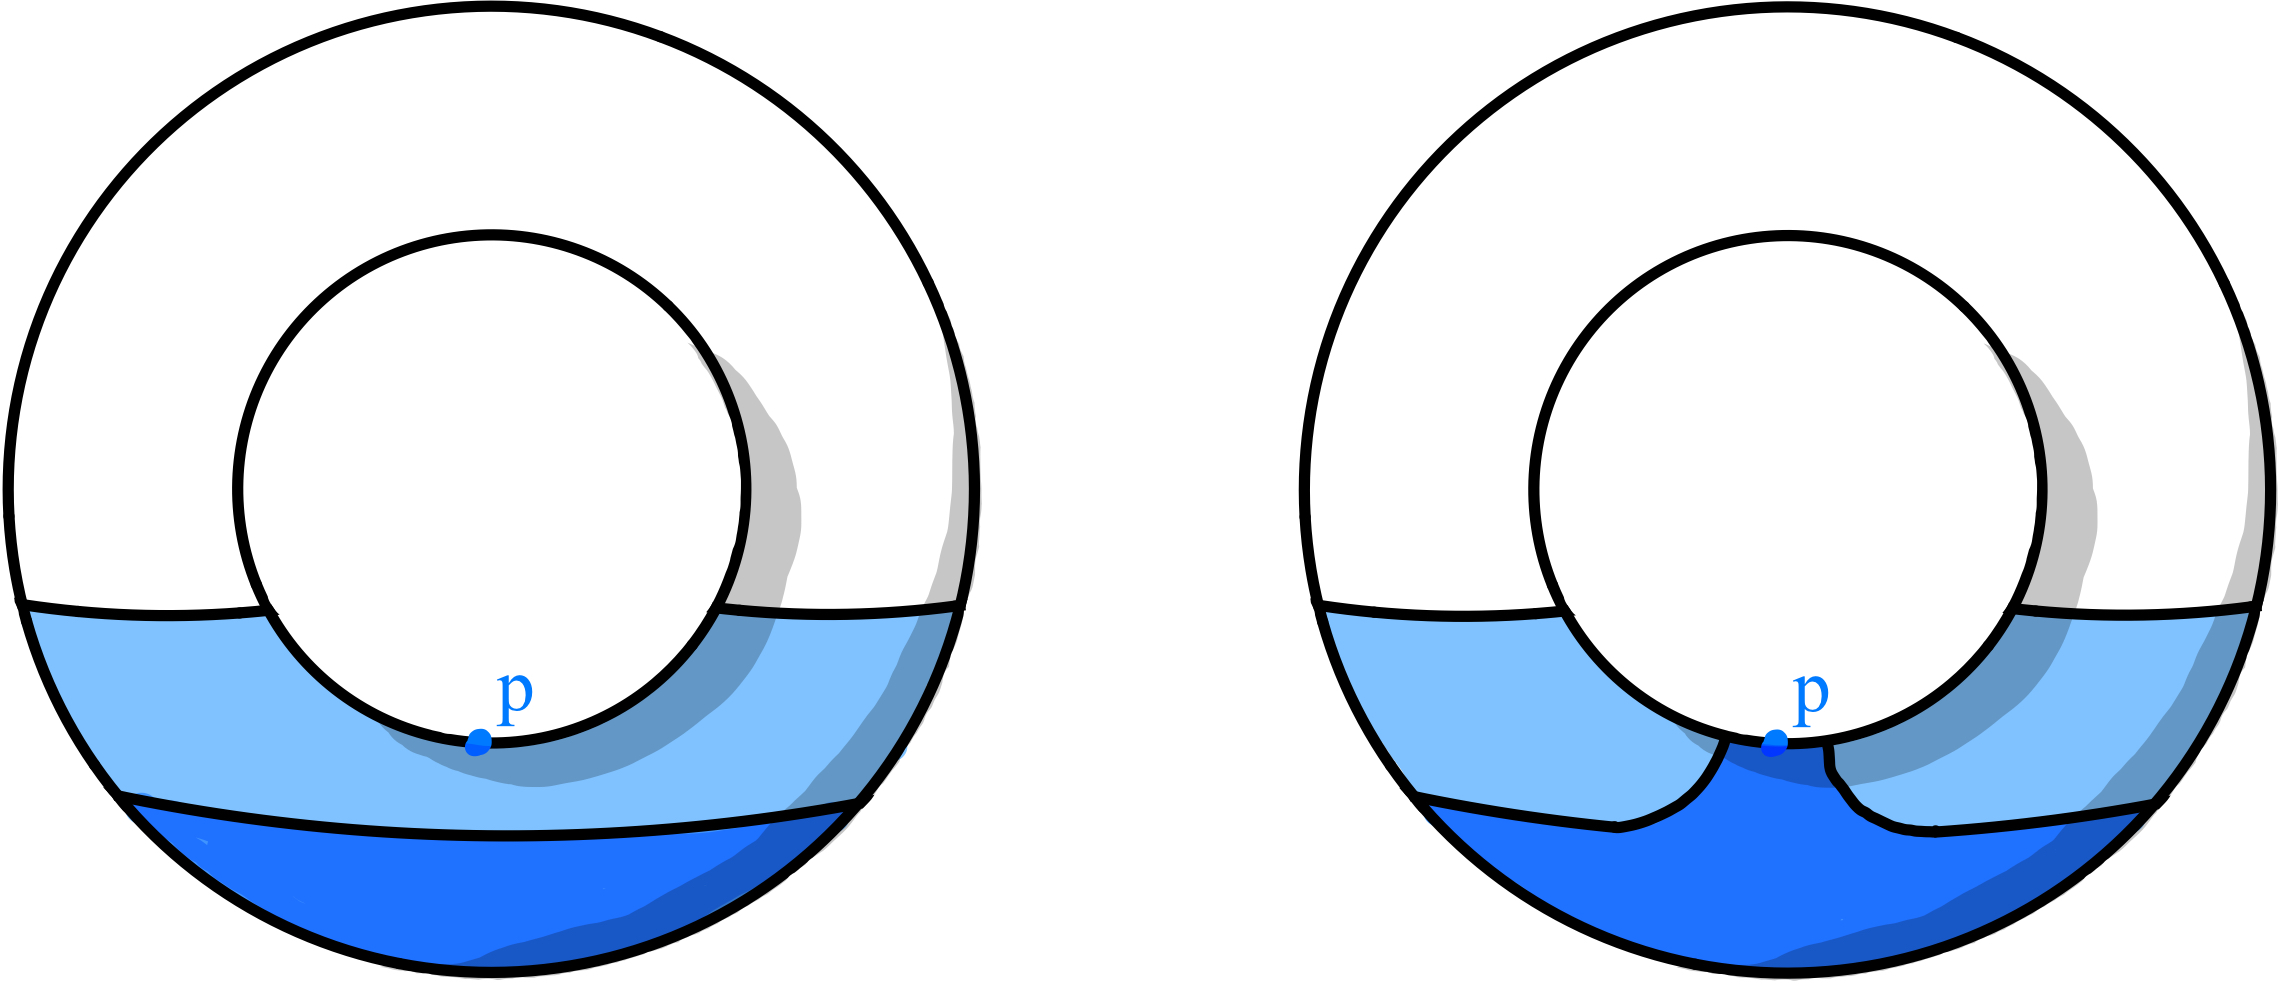
\includegraphics[width=0.8\linewidth]{resources/Me-Diagram5-sublevelsets-of-f-and-F.jpeg}
    \label{fig:me-diagram5}
    \caption{Die Niveaumengen von $f$ (links) und $F$ (rechts)}
\end{figure}

Wir wollen also, dass $M^{c + \varepsilon} = F^{-1}(- \infty, c + \varepsilon]$ 
gilt und $F^{-1}(-\infty, c - \varepsilon]$ fast dasselbe ist wie 
$M^{c - \varepsilon}$, nur dass $F^{-1}(-\infty, c - \varepsilon]$ einen "Henkel"
enthält der den kritischen Punkt $p$ enthält.

\begin{proof}[Beweis zweites Deformationslemma]
    Sei $c := f(p)$. Mit dem Morse-Lemma können wir lokale Koordinaten 
    $\varphi = (u_1, ..., u_n)$ in einer Umgebung $U$ von $p$ wählen, sodass
    \[ f = c - u_1^2 - ... - u_k^2 + u_{k+1}^2 + ... + u_n^2 \]
    in dieser Umgebung, und sodass für den kritischen Punkt $p$ gilt:
    \[ u_1(p) = ... = u_n(p) = 0 \]

    Sei oBdA. $\varepsilon > 0$ klein genug, sodass 
    \begin{enumerate}
        \item $f^{-1}[c - \varepsilon, c + \varepsilon]$ kompakt ist und keine
            kritischen Punkte außer $p$ enthält
        \item $\{ x \in \R^n: \lVert x \rVert^2 \leq 2 \varepsilon \} \subseteq \varphi(U) $
    \end{enumerate}

    Wähle nun die $k$-Zelle 
    \[ 
        e^k := \{ p \in M: (u_1(p))^2 + ... + (u_k(p))^2 \leq \varepsilon 
        \text{ und } u_{k+1}(p) = ... = u_n(p) = 0 \} 
    \]

    Wir bekommen die folgende Situation:

    \begin{figure}[H]
        \centering
        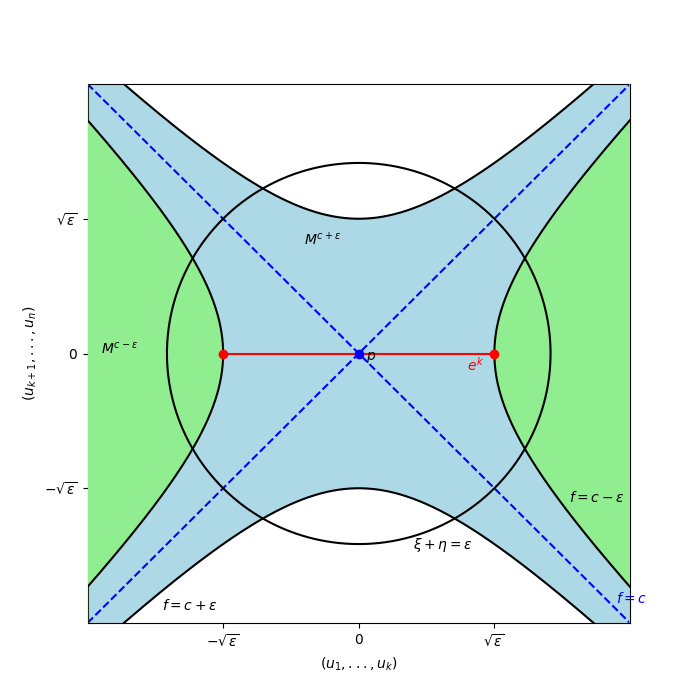
\includegraphics[width=0.8\linewidth]{resources/Me-Diagram6-U-parameterized.png}
        \label{fig:me-diagram6}
        \caption{U parametrisiert}
    \end{figure}

    Nun definiere eine glatte Funktion $\mu: \R \to \R$ mit den Eigenschaften:

    \begin{enumerate}
        \item $ \mu(0) > \varepsilon $
        \item $ \mu(r) = 0 $ falls $ r \geq 2 \varepsilon $
        \item $ -1 < \mu'(r) \leq 0 $ für alle $ r \in \R $
    \end{enumerate}

    Sei nun $F$ außerhalb von $U$ gleich $f$, und sei
    \[ F = f - \mu(u_1^2 + ... + u_k^2 + 2u_{k+1}^2 + ... + 2u_n^2) \]

    $F$ ist wohldefiniert und glatt, da $F$ außerhalb des Kreises mit Radius 
    $\sqrt{2\varepsilon}$ mit $f$ übereinstimmt und der gesamte Kreis in $U$ 
    enthalten ist. Damit haben wir einen guten Kandidaten foür $F$ gefunden.

    Wir definieren nun

    \begin{align*}
        & \eta, \xi: U \to [0, \infty) \\
        & \xi = u_1^2 + ... + u_k^2 \\
        & \eta = u_{k + 1}^2 + ... + e_n^2
    \end{align*}

    Dann gilt innerhalb von $U$:
    \[ f = c - \xi + \eta \]
    und 
    \[ F = f - \mu(\xi + 2 \eta) = c - \xi + \eta - \mu(\xi + 2 \eta) \]

    Jetzt wollen wir überprüfen:
    \begin{enumerate}
        \item $F^{-1}(-\infty, c + \varepsilon] = M^{c + \varepsilon}$.
        \item $F^{-1}(-\infty, c - \varepsilon]$ ist ein Deformationsretrakt von 
            $M^{c + \varepsilon}$.
        \item $M^{c - \varepsilon} \cup e^k$ ist ein Deformationsretrakt von
            $F^{-1}(-\infty, c - \varepsilon]$.
    \end{enumerate}

    Dann folgt schon die Behauptung.

    \proofheading{Behauptung 1} $F^{-1}(-\infty, c + \varepsilon] = M^{c + \varepsilon}$

    Sei $q \in M$. Falls gilt $\xi(q) + 2 \eta(q) > 2 \varepsilon$ gilt 
    $F(q) = f(q) - \mu(\xi(q) + 2\eta(q)) = f(q)$,
    also gelte oBdA.
    \[ \xi(q) + 2 \eta(q) \leq 2 \varepsilon \]
    Dann:
    \[ F(q) \leq f(q) = c - \xi(q) + \eta(q) \leq c + \frac{1}{2}\xi(q) + \eta(q) \leq c + \varepsilon \]
    \sectiondone

    \proofheading{Behauptung 2} $F^{-1}(-\infty, c - \varepsilon]$ ist ein
    Deformationsretrakt von $M^{c + \varepsilon}$.

    Bemerke: Die kritischen Punkte von $F$ stimmen mit denen von $f$ überein, 
    denn:

    \[ \pderive[F]{\xi} = -1 - \mu'(\xi + 2\eta)  < 0 \]
    und
    \[ \pderive[F]{\eta} = 1 - 2 \mu'(\xi + 2\eta) \geq 1 \]
    Insbsondere sind diese beiden Ableitungen also niemals $0$. Da 
    \[ \opd F = \pderive[F]{\xi}\opd \xi + \pderive[F]{\eta} \opd \eta \]
    und $\opd \xi$ und $\opd \eta$ nur in $p$ gleichzeitig Null sind, haben $f$ 
    und $F$  dieselben kritischen Punkte.

    Betrachte die Region $F^{-1}[c - \varepsilon, c + \varepsilon]$. Wegen 
    Behauptung 1 und der Tatsache, dass $F \leq f$ gilt:
    \[ F^{-1}[c - \varepsilon, c + \varepsilon] \subseteq f^{-1}[c - \varepsilon, c + \varepsilon] \]
    Da $f^{-1}[c - \varepsilon, c + \varepsilon]$ kompakt ist und 
    $F^{-1}[c - \varepsilon, c + \varepsilon]$ abgeschlossen ist, ist 
    $F^{-1}[c - \varepsilon, c + \varepsilon]$ auch kompakt. Da $f$ und $F$
    dieselben kritischen Punkte haben kann diese Menge maximal den kritischen 
    Punkt $p$ enthalten, aber
    \[ F(p) = c - \xi(p) + \eta(p) + \mu(\xi(p) + 2\eta(p)) = c - \mu(0) < c - \varepsilon \]
    Also gibt es in $F^{-1}[c - \varepsilon, c + \varepsilon]$ keine kritischen
    Punkte. Mit dem ersten Deformationslemma gilt dann:
    $F^{-1}(- \infty, c - \varepsilon]$ ist Def. Retrakt von 
    $F^{-1}(-\infty, c + \varepsilon] = M^{c + \varepsilon}$.
    \sectiondone

    \proofheading{Behauptung 3} $M^{c - \varepsilon} \cup e^{k}$ ist ein 
    Deformationsretrakt von $F^{-1}(-\infty, c - \varepsilon]$.

    Diese Aussage ergibt nur Sinn, falls 
    $M^{c - \varepsilon} \cup e^{k} \subseteq F^(-\infty, c - \varepsilon]$.
    Wir wissen schon, dass $M^{c - \varepsilon} \subseteq F^{-1}(c - \varepsilon]$.

    Sei $q \in e^k$, dann gilt $\xi(p) = 0 \leq \xi(q) \leq 1$ und 
    $\eta(p) = 0 = \eta(q)$. Da 
    $\pderive[F]{\xi} < 0$ gilt dann
    \[ F(q) \leq F(p) < c - \varepsilon \]

    Also ergibt sich folgende Situation:

    \begin{figure}[H]
        \centering
        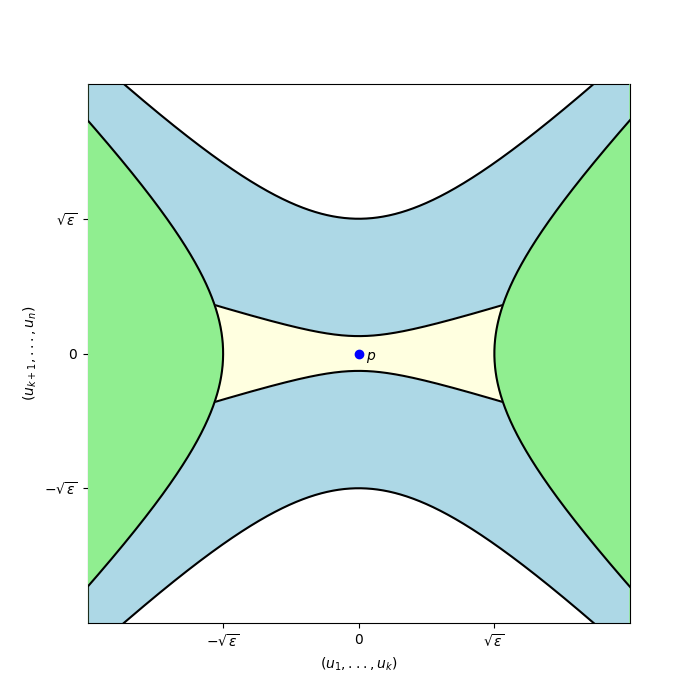
\includegraphics[width=0.8\linewidth]{resources/Me-Diagram7-handle.png}
        \label{fig:me-diagram7}
        \caption{Henkel}
    \end{figure}

    Die hellgrün eingefärbte Fläche ist $M^{c - \varepsilon}$ die hellgelbe
    zusammen mit der hellgrünen Fläch ist $F^{-1}(-\infty, c - \varepsilon]$. 

    Dafür konstruieren wir eine Deformationsretraktion
    $r: F^{-1}(-\infty, c - \varepsilon] \times [0,1] \to F^{-1}(-\infty, c - \varepsilon]$
    für $q \in F^{-1}(-\infty, c - \varepsilon], t \in [0, 1]$, die 
    $F^{-1}(-\infty, c - \varepsilon] - M^{c - \varepsilon}$ auf $e^k$ 
    deformiert, wie folgt.

    \[
        r(q, t) = \begin{cases}
            \varphi^{-1} \circ (u_1, ..., u_k, tu_{k + 1}, ..., tu_n)(q)
                & \text{ im Fall 1: } \xi(q) \leq \varepsilon \\
            \varphi^{-1} \circ (u_1, ..., u_k, s_tu_{k + 1}, ..., s_tu_n)(q)
                & \text{ im Fall 2: } \varepsilon \leq \xi(q) \leq \eta(q) + \varepsilon \\
            q & \text{ im Fall 3: } \eta(q) + \varepsilon \leq \xi(q)
        \end{cases}
    \]

    Wobei 

    \[ s_t = t + (1 -t)((\xi - \varepsilon)/\eta)^{1/2} \]

    Die Fälle sind dann wie folgt:

    \begin{figure}[H]
        \centering
        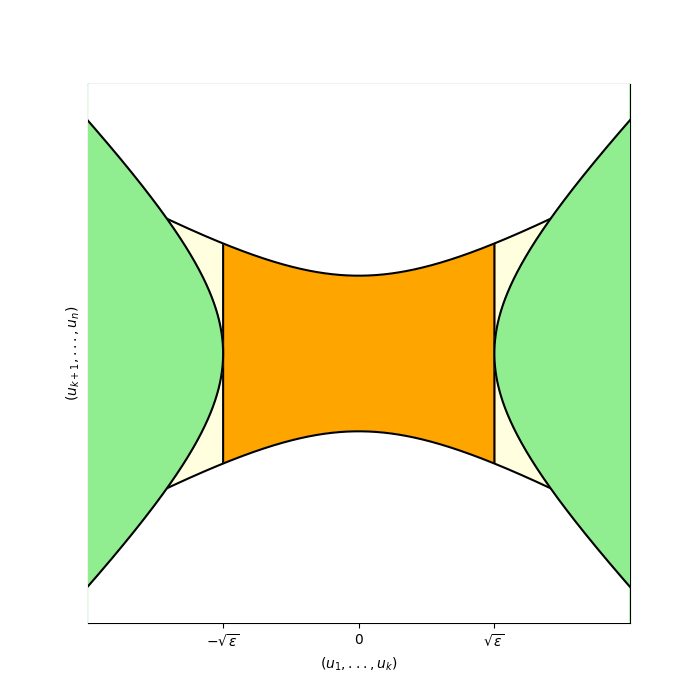
\includegraphics[width=0.8\linewidth]{resources/Me-Diagram9-handle-cases.png}
        \label{me-diagram9}
        \caption{
            Fall 3 ist $M^{c - \varepsilon}$, also die grün eingefärbte Fläche, die
            orangene Fläche ist Fall 1 und die gelbe ist Fall 2.
        }
    \end{figure}

    Wir müssen überprüfen:
    \begin{enumerate}
        \item $r$ ist wohldefiniert und stetig
        \item $r(F^{-1}(-\infty, c - \varepsilon], 0) \subseteq M^{c - \varepsilon} \cup e^k$
        \item $r(\cdot, 1) = \id_{F^{-1}(-\infty, c - \varepsilon]}$ und 
            $\left. r(\cdot , 0) \right\vert_{M^{c - \varepsilon} \cup e^k} 
            = \id_{M^{c - \varepsilon} \cup e^k}$
    \end{enumerate}

    3. ist einfach nachzurechnen. In Fall 1 und Fall 3 ist 2. offensichtlich
    wahr. Für Fall 2 gilt:
    \begin{align*} 
        f(r(0, q)) & = 
            f\left( \varphi^{-1} \left(u_1(q), ..., u_k(q), 
            \left( \frac{\xi(q) - \varepsilon}{\eta(q)} \right)^{1/2}u_{k + 1}(q), ...,
            \left( \frac{\xi(q) - \varepsilon}{\eta(q)} \right)^{1/2}u_n(q)
            \right)
            \right) \\
        & = c - \xi(q)
            + \left( \left( \frac{\xi(q) - \varepsilon}{\eta(q)} \right)^{1/2}u_{k + 1}(q) \right)^2 + ... 
            + \left( \left( \frac{\xi(q) - \varepsilon}{\eta(q)} \right)^{1/2}u_n(q) \right)^2 \\
        & = c - \left( \frac{\xi(q) - \varepsilon}{\eta(q)} \right) \eta(q) \\
        & = c - \varepsilon
    \end{align*}
    also ist $r(0, q) \in f^{-1}(c - \varepsilon)$. Um 1. zu prüfen müssen wir 
    Stetigkeit in den Grenzfällen überprüfen:
    \begin{align*}
        & \text{For } \xi(q) = \varepsilon \text{ : }
            & s_t(q)  =t + (1 - t)((\varepsilon - \varepsilon)/\eta(q))^{1/2} = t \\
        & \text{For } \eta(q) + \varepsilon = \xi(q) \text{ : }
            & s_t(q) = t + (1 - t)((\xi(q) - \varepsilon)/(\xi(q) - \varepsilon))^{1/2} = 1
    \end{align*}

    Das einzig andere Problem was wir bekommen könnten ist nun in Fall 2 falls
    $\eta \to 0$. In Fall 1 und Fall 3 bekommen wir für $q$ mit $\eta(q) = 0$:
    $r(q, t) = \varphi^{-1} \circ (u_1, ..., u_k, 0, ..., 0)(q)$, also wollen
    wir zeigen dass für $\eta \in $ Fall 2 mit $\eta \to 0$ gilt $s_tu_i \to 0$
    für $i \in \{k+1, ..., n\}$. In Fall 2 gilt
    $0 \leq \xi - \varepsilon \leq \eta$. Dann gilt:

    \begin{align*}
        \lim\limits_{\eta \to 0} | s_t u_i |
           & = \lim\limits_{\eta \to 0} (1 - t)((\xi - \varepsilon)/\eta)^{1/2} | u_i | \\
           & \leq \lim\limits_{\eta \to 0} (1 - t)(\eta/\eta)^{1/2}|u_i| \\
           & = \lim\limits_{\eta \to 0} (1 - t)|u_i| = 0 
    \end{align*}
    
    Also ist $r$ stetig.
    \sectiondone

    Mit Behauptung 3 und 4 bekommen wir
    \[ M^{c + \varepsilon} \simeq F^{-1}(c - \varepsilon] \]
    und 
    \[ F^{-1}(-\infty, c - \varepsilon] \simeq M^{c - \varepsilon} \cup e^k \]
    Also folgt die Behauptung:
    \[ M^{c + \varepsilon} \simeq M^{c - \varepsilon} \cup e^k \]

\end{proof}
